\chapter{Statistical mechanics on chygraphs}
\label{ch:statmech}

There is a point in the study of disordered systems at which the model stops
mattering. A magnet, a minimum vertex cover and a random Boolean formula have
nothing in common as subject matter --- one is physics, one is combinatorial
optimisation, one is logic --- and the same recursion solves all three. It has
been rediscovered often enough to have collected a name in each field: the
Bethe--Peierls approximation, the cavity method, belief propagation. What
distinguishes the three problems is not the recursion. It is only what one
message is required to carry: a number, a distribution, a warning.

This chapter takes that observation seriously enough to write it down once.

Chapter~\ref{ch:potts} claimed that percolation and the Ising model are one
recursion at two values of a parameter, and checked it at both values. That is a
claim about two special cases. This chapter writes the recursion down for
an arbitrary interaction inside a complex, so that the claim stops being about
special cases and becomes the method. Nothing in the chapter has appeared
elsewhere.

The generalisation is one substitution, and Sec.~\ref{sec:substitution} states
it before anything else, because everything afterwards is bookkeeping around
it. The bookkeeping is done once here: the same two steps,
the same branching matrix and the same free energy serve
Chapters~\ref{ch:ising}--\ref{ch:satisfiability} without being rederived.

\section{One substitution}
\label{sec:substitution}

Percolation's message was a number: $Q^{ml}_{i}$, the probability that an
inclusion leads nowhere. The map, Eqs.~\eqref{eq:Qminus}--\eqref{eq:Qplus},
combined those numbers by evaluating generating functions at them and
multiplying.

For a general model the message is a \emph{cavity field} --- how strongly one
part of the chygraph tells another to point up rather than down --- and, at the
level of an ensemble rather than one realisation, a whole distribution of
cavity fields. So make one substitution:

\begin{center}
\emph{the argument of a generating function becomes a measure,\\
and the product becomes a convolution.}
\end{center}

Concretely, let a generating function act on a measure by
\begin{equation}
  \Phi^{l}_{k}\ast Q=\sum_{n}p^{lk}_{n}\,Q^{\ast n},
  \qquad
  \Phi^{l}_{k}(x)=\sum_{n}p^{lk}_{n}x^{n},
  \label{eq:conv}
\end{equation}
the $n$-fold convolution weighted by the chy-degree distribution. Writing
$Q^{lk}$ for the law of the field a layer-$k$ complex emits onto a layer-$l$
complex, the law $P^{ml}$ of the field a layer-$l$ complex sends up into a
layer-$m$ complex is
\begin{equation}
  P^{ml}=\delta_{B}\ast\Bigl(\ast_{k}\,
    \bigl[\bar\Phi^{l}_{k}\bigr]_{k=m}\!\ast\,Q^{lk}\Bigr),
  \label{eq:ensemblemap}
\end{equation}
with $\delta_{B}$ the point mass at the external field $B$ --- the letter
Eq.~\eqref{eq:Hising} uses, and the branching matrix below is the only other
$B$ in the chapter, always either carrying two layer indices or standing inside
$\det(I-B)$ --- and
$[\bar\Phi]_{k=m}$ the same bracket as Fig.~\ref{fig:themap} --- excess on the
layer arrived through, ordinary on every other. Nothing else about
Chapter~\ref{ch:percolation}'s index structure has changed. The layers, the
directions of arrival, the discounting of the inclusion one came in by: all of
it survives verbatim, because none of it was about what the message contained.

Two sanity checks come for free, and they say what the substitution costs.

Put $Q^{lk}=\delta_{u}$, a point mass at a single number. Every convolution
collapses to a product and Eq.~\eqref{eq:ensemblemap} \emph{is} the percolation
map. Percolation is the case in which no distribution is needed, which
Chapter~\ref{ch:potts} explained: at $q=1$ the number is a probability and the
composition is multiplication.

And the first moment of a convolution is the sum of the first moments of its
factors. So linearising Eq.~\eqref{eq:ensemblemap} about the trivial fixed
point gives a linear operator with the same index structure as
Sec.~\ref{sec:threshold}'s tensor --- which is Sec.~\ref{sec:branching}, and it
is why the threshold calculation of Part~II is reusable rather than merely
analogous.

\section{The two steps}
\label{sec:twosteps}

A message lives on a directed inclusion and is updated from every incoming
message except the one it came from. On a chygraph that update has two halves,
and they are of quite different character (Fig.~\ref{fig:twosteps}).

\subsection{Up: a convolution}
\label{sec:upstep}
\index{convolution}

On one realisation, what a node tells a complex it belongs to is the sum of
what its \emph{other} complexes have told it:
\begin{equation}
  h_{i\to a}=B+\sum_{b\ni i,\ b\ne a}u_{b\to i}.
  \label{eq:up}
\end{equation}
Fields add. That is the up step, and it is why the ensemble
version, Eq.~\eqref{eq:ensemblemap}, is a convolution: the law of a sum of
independent terms is the convolution of their laws, and the generating function
supplies how many terms there are.

Equation~\eqref{eq:up} is also where the treelike assumption sits, ahead of
Sec.~\ref{sec:assumes}. Adding the $u_{b\to
i}$ independently is exact only if the complexes at $i$ carry independent
information --- if they meet only at $i$. Section~\ref{sec:treelike} said what
that costs and Chapter~\ref{ch:overlap} pays it.

\subsection{Down: an exact sum inside the complex}
\label{sec:downstep}
\index{interior sum|textbf}

The other half is where percolation and statistical mechanics part company. For
a complex holding $c$ members with internal energy $-\beta H(\sigma)$, the field
it emits onto member $0$ given the cavity fields of the others is
\begin{equation}
  \begin{split}
    u&=\tfrac12\ln\frac{\bar{Z}(\sigma_{0}=+1)}{\bar{Z}(\sigma_{0}=-1)},\\
    \bar{Z}(\sigma_{0})&=\!\!\sum_{\sigma_{1}\dots\sigma_{c-1}}\!\!
      e^{-\beta H(\sigma)+\sum_{j}h_{j}\sigma_{j}}.
  \end{split}
  \label{eq:emitted}
\end{equation}
That sum is done \emph{exactly}, at a cost exponential in $c$ and independent of
everything outside the complex.

Equation~\eqref{eq:emitted} reads like a definition and is not. What the complex
has to tell member $0$ is the whole of its effect on that member, which is the
function $\hat\nu(\sigma_{0})\propto \bar{Z}(\sigma_{0})$. A function of one Ising
variable takes two values, and only their ratio is used, because the message
enters a normalised measure. So the message is one number however large the
complex is --- the enumeration behind it grows as $2^{c}$, what comes out of it
does not --- and writing that number in the exponential form the up step needs,
$\hat\nu(\sigma_{0})\propto e^{u\sigma_{0}}$, fixes $e^{u}/e^{-u}=\bar{Z}(+1)/\bar{Z}(-1)$,
which is Eq.~\eqref{eq:emitted}. The $\tfrac12$ is there because
$\sigma_{0}=\pm1$ rather than $0,1$. It is the same parameterisation that makes
Eq.~\eqref{eq:up} a sum: messages compose by multiplication, and $h$ is the
exponent in which multiplication is addition.

At $c=2$ this returns what Chapter~\ref{ch:introduction} already had. One other
member and one bond give
\begin{align*}
  \bar{Z}(\sigma_{0})&=\sum_{\sigma_{1}}
    e^{\beta J\sigma_{0}\sigma_{1}+h_{1}\sigma_{1}}
    =2\cosh(\beta J\sigma_{0}+h_{1}),\\
  u&=\tfrac12\ln\frac{\cosh(\beta J+h_{1})}{\cosh(\beta J-h_{1})}
   =\mathrm{atanh}\bigl[\tanh\beta J\,\tanh h_{1}\bigr],
\end{align*}
which is the link message of Sec.~\ref{sec:cavity}, and near $h_{1}=0$ it is
$u\simeq t\,h_{1}$ with $t=\tanh\beta J$. That comparison also fixes the units,
which change here and are worth stating once: in Chapter~\ref{ch:introduction} a
field is an energy and $\beta$ is written out, while from
Eq.~\eqref{eq:emitted} onwards it is absorbed, the $h$ here being the $\beta h$
there. Absorbing it is what lets $u'$ below be a pure number. The interior sum
itself, for any $-\beta H$, is \code{cavity.\allowbreak emitted\_\allowbreak field}.

Three properties of Eq.~\eqref{eq:emitted} carry the chapter.

\emph{The Hamiltonian appears here and nowhere else.} Everything upstream and
downstream is structure. Changing the model means passing a different
$-\beta H$ to one routine, which is why Chapters~\ref{ch:ising}
to~\ref{ch:cover} are substitutions rather than derivations, and why the
unanimity interaction of Sec.~\ref{sec:unanimity} needed nothing new.

\emph{Percolation could compress this and a general model cannot.} Reachability
factorises --- whether $i$ reaches $j$ inside the complex does not depend on
what happens outside it --- so Chapter~\ref{ch:percolation} could reduce the
whole interior to one component-size generating function $\bar G$. An
interaction does not factorise and has to be summed. Chapter~\ref{ch:potts}
made this precise from the other side: Eq.~\eqref{eq:qonelimit} is exactly the
statement that the sum \emph{becomes} $\bar G$ as $q\to1$.

\emph{This is what promoting a motif to a complex buys.} A triangle treated as
three links is a loop and breaks the tree assumption. A triangle treated as one
complex has its loop \emph{inside} Eq.~\eqref{eq:emitted}, where it is summed
over exactly and nothing outside ever learns it was there. The price is $2^{c}$,
and for the motifs one actually finds in data --- Chapter~\ref{ch:data}'s
cliques run to a handful of members --- that price is nothing.

\begin{figure}[t]
\centering
\begin{adjustbox}{max width=0.98\linewidth}
\begin{tikzpicture}
% Node i sits in two complexes, which meet only at i. Up is a sum over the
% others; down is an enumeration inside one of them. The two complexes carry
% different greys so that the shared node reads as a meeting point rather than
% as the overlap of Ch. 13, which is drawn in one grey on purpose.
\node[hub] (i) at (0,0) {};
\node[lb,anchor=north west] at (0.13,-0.10) {$i$};
% complex a, above: its interior is drawn, because the interior is the point
\node[nd] (a1) at (-0.95,1.45) {};
\node[nd] (a2) at (0.95,1.45) {};
\draw[lnk] (i)--(a1) (i)--(a2) (a1)--(a2);
\begin{scope}[on background layer]
  \node[cx,fit=(i)(a1)(a2)] (A) {};
\end{scope}
\node[lb,anchor=south] at (0,1.90) {complex $a$, cardinality $c$};
% complex b, below
\node[nd] (b1) at (-0.95,-1.45) {};
\node[nd] (b2) at (0.95,-1.45) {};
\draw[lnk] (i)--(b1) (i)--(b2) (b1)--(b2);
\begin{scope}[on background layer]
  \node[cxb,fill opacity=0.72,fit=(i)(b1)(b2)] (B) {};
\end{scope}
\node[lb,anchor=north] at (0,-1.90) {complex $b$};
% the two messages, on the a side
\draw[msg] (-0.26,0.24) -- (-0.66,1.06);
\node[lb,anchor=east] at (-0.70,0.62) {$h_{i\to a}$};
\draw[msg] (0.66,1.06) -- (0.26,0.24);
\node[lb,anchor=west] at (0.70,0.62) {$u_{a\to i}$};
% what each step is
\node[lb,anchor=west,align=left] at (2.20,0.85)
  {\emph{up}, Eq.~\eqref{eq:up}:\\
   $h_{i\to a}$ adds what every\\
   \emph{other} complex told $i$.\\
   A sum --- so a convolution\\
   over an ensemble};
\node[lb,anchor=west,align=left] at (2.20,-0.85)
  {\emph{down}, Eq.~\eqref{eq:emitted}:\\
   $u_{a\to i}$ enumerates the\\
   $2^{c}$ interior states of $a$.\\
   The only place the\\
   Hamiltonian appears};
\end{tikzpicture}
\end{adjustbox}
\caption{\textbf{The two steps.} A node passes up the sum of what its other
complexes have told it, Eq.~\eqref{eq:up}; a complex passes down the field
implied by an exact enumeration of its own interior, Eq.~\eqref{eq:emitted}.
The asymmetry is the content. The up step knows nothing of the model and the
down step knows nothing of the rest of the chygraph, so a new model changes one
routine and a new structure changes the other, and neither disturbs the other.
Compare Fig.~\ref{fig:themap}, which is this picture with a number in place of
each message.}
\label{fig:twosteps}
\end{figure}

\section{The branching matrix}
\label{sec:branching}
\index{branching matrix|textbf}

The transition follows from linearising both steps about the trivial fixed
point, where every field vanishes. The down step, Eq.~\eqref{eq:emitted},
responds to each of the complex's other members separately and, at that point,
with the same derivative for each, the interior being symmetric under permuting
them:
\begin{equation}
  \delta u_{a\to i}=u'\!\!\sum_{j\in a\setminus i}\!\delta h_{j\to a},
  \qquad
  u'=\frac{\partial u}{\partial h}\bigg|_{\text{trivial}}.
  \label{eq:uprime}
\end{equation}
The up step, Eq.~\eqref{eq:up}, then adds what the node's other complexes have
sent, $\delta h_{i\to a}=\sum_{b\ni i,\,b\ne a}\delta u_{b\to i}$. Composing
the two, a perturbation is multiplied by $u'$ once per complex traversed and
fanned out twice: over the $c-1$ other members of that complex, and over the
other complexes at the node it lands on. Only the first of the three factors
knows the model. So every traversal of a complex carries one number, $u'$, and
nothing else of the interaction survives the linearisation; the two counting
factors are structure, and assembling them is all
Eqs.~\eqref{eq:branch}--\eqref{eq:sbaru} below do.

That number has been met already. It is Chapter~\ref{ch:potts}'s transmission
$\tau_{c}$, Eq.~\eqref{eq:taudef}, for the case where the interior is a Potts
interaction --- the same derivative of the same emitted quantity at the same
fixed point. For the Ising interaction of Chapter~\ref{ch:ising} it is
$\tau_{c}(2,v)$, verified for $c=2,3,4$: $u'=t$, $t/(1-t+t^{2})$ and
$(t+t^{3})/(1-2t+3t^{2})$ with $t=\tanh\beta J$.

\paragraph{Reusing the threshold tensor.} Because $u'$ enters as a single factor
per traversal, the whole apparatus of Sec.~\ref{sec:threshold} applies to any
model with one substitution,
\begin{equation}
  \ave{s}\ \longrightarrow\ \ave{s\,u'},
  \qquad
  \ave{\sbar}\ \longrightarrow\ \ave{\sbar\,u'},
  \label{eq:reweight}
\end{equation}
an elementwise reweighting that leaves the index structure, the block layout
and the determinant untouched. The weight belongs on the intra-complex channel,
because the interaction lives inside a complex; the chy-degree step is a relay
and carries weight one, so $\ave{\kappa}$ and $\ave{\kbar}$ are left alone.
Replacing $u'$ by $u'^{2}$ throughout gives
the de Almeida--Thouless line instead of the ferromagnetic one, which is
Chapter~\ref{ch:ising}'s spin-glass boundary for the price of a square.

\paragraph{The matrix.} Collecting the two steps: arriving at a node through a
layer-$l$ complex, it belongs to $\ave{\kbar}_{m}$ further layer-$m$ complexes
when $m=l$ and $\ave{\kappa}_{m}$ otherwise --- Chapter~\ref{ch:percolation}'s
bracket again --- and each such complex offers some number of other members,
each carrying $u'$. So the branching matrix on the $L$ complex layers is
\begin{equation}
  B_{lm}=\Bigl[\ave{\kbar}_{m}\delta_{lm}
              +\ave{\kappa}_{m}(1-\delta_{lm})\Bigr]
         \bigl\langle \sbar\,u'\bigr\rangle_{m},
  \label{eq:branch}
\end{equation}
\begin{equation}
  \bigl\langle \sbar\,u'\bigr\rangle_{m}
    =\sum_{c}\frac{c\,p^{(m)}_{c}}{\ave{c}_{m}}\,(c-1)\,u'(c),
  \label{eq:sbaru}
\end{equation}
and the transition is at
\begin{equation}
  \det\bigl(I-B\bigr)=0.
  \label{eq:det}
\end{equation}

The linear algebra is $L\times L$ however large the complexes are. Cardinality
enters only through Eq.~\eqref{eq:sbaru}, and the number of layers is two or
three for everything in this book. Doing the interior sum locally is what buys
that: it is expensive, and its expense never propagates.

When a layer carries a single cardinality $c_{m}$ --- which is how every layer
in Chapters~\ref{ch:ising}--\ref{ch:cover} is built ---
Eq.~\eqref{eq:sbaru} collapses and
\begin{equation}
  B_{lm}=\Bigl[\ave{\kbar}_{m}\delta_{lm}
              +\ave{\kappa}_{m}(1-\delta_{lm})\Bigr](c_{m}-1)\,u'_{m}.
  \label{eq:branchsingle}
\end{equation}
For one layer this is $(c-1)\,u'\ave{\kbar}=1$, which is
Eq.~\eqref{eq:branchcond} --- the condition Chapter~\ref{ch:potts} wrote down
and deferred to here.

A complex is not sampled uniformly when it is reached by following one of its
inclusions. A complex of cardinality $c$ has $c$ inclusions, so it is reached
$c$ times as often as one of cardinality $1$, and the ensemble seen on arrival
is the size-biased one, $c\,p_{c}/\ave{c}$. Every per-complex quantity in
Eq.~\eqref{eq:branch} is averaged that way.

Taking $f(c)=c-1$ gives the mean number of \emph{other} members on arrival,
\[
  \ave{\sbar}=\sum_{c}\frac{c\,p_{c}}{\ave{c}}(c-1)
             =\frac{\ave{c^{2}}}{\ave{c}}-1,
\]
which is not $\ave{c}-1$. For a layer mixing $c=3$ and $c=5$ in equal
proportion the two are $3.25$ and $3$.

And $\ave{\sbar\,u'}\ne\ave{\sbar}\ave{u'}$ unless $u'$ is common to the layer,
which is why Eq.~\eqref{eq:sbaru} averages the product. For that same layer at
its own critical coupling the two are $0.2500$ and $0.2453$, a difference of
$1.9$ per cent.

Two checks pin this down. Splitting a mixed layer into one layer per
cardinality, with chy-degrees in the ratio $c\,p_{c}$, must give the same
transition, and does: for the $3$-and-$5$ layer at $\ave{\kappa}=4$, both routes
return $T_{c}=15.3758$. Replacing the layer by its mean cardinality must not,
and does not: $T_{c}=13.8218$, low by $10.1$ per cent. A mean cardinality is the wrong
summary of a layer, and Eq.~\eqref{eq:sbaru} is the right one. \code{api.\allowbreak Chygraph.\allowbreak transmission} is Eq.~\eqref{eq:sbaru}, and it averages the product rather than multiplying the averages.

\section{Structures}
\label{sec:structures}
\index{threshold tensor}

Everything above is fixed once the layers, their cardinalities and the
chy-degree distribution are given. Each specialisation below is
Eq.~\eqref{eq:branch} written out, with only $u'$ left for
Eq.~\eqref{eq:emitted} to supply (Table~\ref{tab:structures}).

\begin{table}[b]
\centering\small
\begin{adjustbox}{max width=\linewidth}
\begin{tabular}{ll}
\hline\hline
structure & transition\\
\hline
graph & $\ave{\kbar}\,u'=1$\\[2pt]
clique network, uniform hypergraph & $\ave{\kbar}\,(c-1)\,u'=1$\\[2pt]
mixed cardinalities & $\ave{\kbar}\,\ave{\sbar u'}=1$, Eq.~\eqref{eq:sbaru}\\[2pt]
links and triangles & Eq.~\eqref{eq:LT}\\[2pt]
correlated layers & Eq.~\eqref{eq:LT} with $\ave{\kbar}$ from Eq.~\eqref{eq:biased}\\
\hline\hline
\end{tabular}
\end{adjustbox}
\caption{\textbf{One condition, written out.} Each row is
Eq.~\eqref{eq:branch} for a structure of Sec.~\ref{sec:everything}, and each
needs $u'$ from an enumeration of the interior and nothing else. The
corresponding rows of Chapter~\ref{ch:percolation} are the same expressions
with $u'$ replaced by an occupation probability.}
\label{tab:structures}
\end{table}

A \emph{graph} is one layer of cardinality two and Eq.~\eqref{eq:branch}
collapses to the scalar $\ave{\kbar}u'=1$.

A \emph{clique network or uniform hypergraph} is one layer of cardinality $c$,
giving $\ave{\kbar}(c-1)u'=1$. Cardinality enters twice and the two entrances
are distinct: as the number of other members a complex supplies, and through
$u'$, which depends on $c$ because the interior does. Keeping them apart is
what Chapter~\ref{ch:ising}'s headline result turns on.

\emph{Links and triangles} is two layers, of cardinalities two and three. By
Eq.~\eqref{eq:branchsingle} the four entries are
\[
  \begin{aligned}
    B_{||}&=\ave{\kbar}_{|}u'_{|}, &\quad
    B_{\triangle\triangle}&=2\ave{\kbar}_{\triangle}u'_{\triangle},\\
    B_{|\triangle}&=2\ave{\kappa}_{\triangle}u'_{\triangle}, &\quad
    B_{\triangle|}&=\ave{\kappa}_{|}u'_{|},
  \end{aligned}
\]
the diagonal carrying excess chy-degrees and the off-diagonal ordinary ones,
because a step that arrives from the \emph{other} layer has discounted nothing
in the layer it lands in. Then
$\det(I-B)=(1-B_{||})(1-B_{\triangle\triangle})-B_{|\triangle}B_{\triangle|}$,
and setting it to zero gives
\begin{equation}
  \ave{\kbar}_{|}u'_{|}+2\ave{\kbar}_{\triangle}u'_{\triangle}
  +2u'_{|}u'_{\triangle}\bigl(\ave{\kappa}_{|}\ave{\kappa}_{\triangle}
    -\ave{\kbar}_{|}\ave{\kbar}_{\triangle}\bigr)=1.
  \label{eq:LT}
\end{equation}
The cross term carries
$\ave{\kappa}_{|}\ave{\kappa}_{\triangle}-\ave{\kbar}_{|}\ave{\kbar}_{\triangle}$
and so vanishes whenever both layers are Poisson, each being its own excess. It
does not vanish for regular layers, where $\ave{\kbar}=\ave{\kappa}-1$ and the
coefficient is $\ave{\kappa}_{|}+\ave{\kappa}_{\triangle}-1$. At
$\ave{\kappa}_{|}=4$ and $\ave{\kappa}_{\triangle}=2$ that is $5$, and the two
ensembles have $T_{c}=8.4256$ and $6.8801$. The gap of $1.55$ between them is a
residue and not a sum. The excess chy-degrees alone --- a regular layer having
$\ave{\kbar}=\ave{\kappa}-1$ where a Poisson one is its own excess --- would
take $8.4256$ down to $5.2951$; the cross term carries it back up by $1.58$, and
what survives is the difference. So deleting that one term from the regular case
moves $T_{c}$ by $23$ per cent, more than the whole distance between the two
ensembles it is a correction to. It is one term, and it is easy to drop.

\emph{Correlated layers} are Sec.~\ref{sec:joint} unchanged: replace the
marginals by a joint $\Phi$ and $\ave{\kbar}$ by the inclusion-biased second
moment of Eq.~\eqref{eq:biased}. Nothing else in Eq.~\eqref{eq:branch} moves,
which is the same statement Chapter~\ref{ch:giant} made for percolation and for
the same reason.

\section{Away from the trivial fixed point}
\label{sec:fixedpoint}

Equation~\eqref{eq:branch} is the Jacobian of the map at its \emph{trivial}
fixed point, and Sec.~\ref{sec:jacobian} already established what that means for
percolation: its Perron root is $1+\Lambda$. Evaluating the same Jacobian at the
fixed point the map actually reaches answers a different question --- whether the
solution found is locally stable --- and the two answers are related.

For percolation,
\begin{equation}
  \rho\bigl(J(Q^{*})\bigr)=1-\Lambda+O(\Lambda^{2}),
  \label{eq:exchange}
\end{equation}
the two roots leaving $1$ at the same rate in opposite directions
(Fig.~\ref{fig:exchange}). An exchange of stability, and made quantitative
rather than asserted: for a Poisson graph the residual $1-\rho-\Lambda$ falls
from $-7.4\times10^{-5}$ at $\Lambda=1.5\times10^{-2}$ to $-8.3\times10^{-8}$ at
$\Lambda=5.0\times10^{-4}$, and divided by $\Lambda^{2}$ it settles at $-0.333$.
For a Poisson hypergraph it settles at $-0.629$. Dividing by $\Lambda^{2}$ is
what fixes the order at quadratic; a single point could only have bounded it.
Closer in than this the residual reaches $10^{-8}$ and rounding takes over, so
the sequence is stopped before it does.

\begin{figure}[t]
\centering
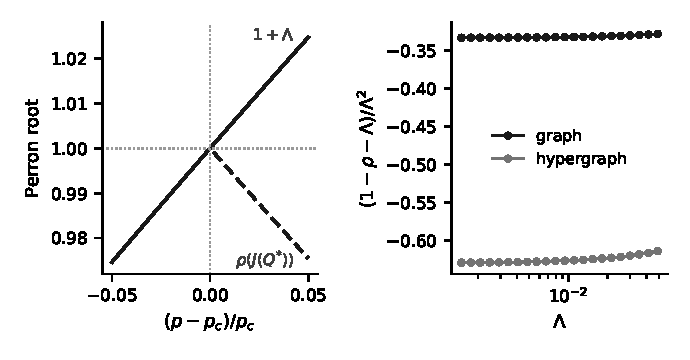
\includegraphics[width=\linewidth]{figs/fig-exchange.pdf}
\caption{\textbf{An exchange of stability.} Left: the Perron root of the
Jacobian at the trivial fixed point, $1+\Lambda$, and at the fixed point the map
reaches, for site percolation on a Poisson graph with $\ave{k}=3$. Where the
first passes through $1$ the second leaves it, at the same rate. Right: what is
left after the linear term, $(1-\rho-\Lambda)/\Lambda^{2}$, for that graph and
for a Poisson hypergraph with $\ave{k}=2$, $\ave{c}=3$. It settles at a constant,
so Eq.~\eqref{eq:exchange}'s remainder is quadratic; the constant is
model-dependent and the linear term is not. Generated by
\code{figs/\allowbreak statmech.\allowbreak py}.}
\label{fig:exchange}
\end{figure}

\paragraph{One diagnostic does not survive the move.} It is the natural thing
to reach for and it is wrong. The sign of the
leading eigenvalue does \emph{not} distinguish an order-preserving map from an
order-reversing one. The coupled core of a chygraph alternates between the up
and down roles of Eqs.~\eqref{eq:up} and~\eqref{eq:emitted}, so $J$ is a
non-negative matrix of period two, and Perron--Frobenius then places eigenvalues
at both $+\rho$ and $-\rho$. A negative leading eigenvalue is the geometry of
the chygraph, not a statement about the map.

The unambiguous test is the sign of the \emph{entries}: non-negative for a map
built from generating functions, non-positive for the hard-core maps of
Chapter~\ref{ch:hittingset}. That distinction decides which solver applies ---
plain iteration converges for one and oscillates forever for the other --- and
Chapter~\ref{ch:hittingset} turns on it.

\section{Free energy}
\label{sec:freeenergy}
\index{Bethe free energy|textbf}

A linear instability locates a transition only when the transition is
continuous. Chapter~\ref{ch:potts} met that limit at $q>2$,
Chapter~\ref{ch:giant} met it for interdependent networks and
Chapter~\ref{ch:epidemics} for threshold contagion, and
Chapter~\ref{ch:ising} will meet it again. In every case what is needed instead
is a free energy, so this chapter has to supply one.

The general Bethe free energy is Eq.~\eqref{eq:bethe-intro} with a complex in
place of a link: one term per complex, one per node, and one subtracted per
inclusion,
\[
  -\beta f=\sum_{a}\ln Z_{a}+\sum_{i}\ln Z_{i}
           -\sum_{(ia)}\ln Z_{ia},
\]
the last removing what the first two count twice. Parameterise the messages as
$\nu_{i\to a}(\sigma)\propto e^{h_{i\to a}\sigma}$ and
$\hat\nu_{a\to i}(\sigma)\propto e^{u_{a\to i}\sigma}$. The overlap term then
collapses, for a reason specific to this
parameterisation: $h_{i\to a}+u_{a\to i}$ is the \emph{same} full field $h_{i}$
for every complex $a$ containing $i$, so the overlaps do not depend on which
complex is being subtracted. What is left is one term per complex and $1-k_{i}$
per node,
\begin{equation}
  -\beta f=\sum_{l}n_{l}\ave{\ln Z^{(l)}_{a}}+\ave{(1-\kappa)\ln Z_{i}},
  \qquad
  n_{l}=\ave{\kappa_{l}}/c_{l},
  \label{eq:bethe}
\end{equation}
with $Z_{a}$ the exact partition function inside a complex --- the same
enumeration as Eq.~\eqref{eq:emitted}, reused --- and $Z_{i}=2\cosh h_{i}$. At
zero cavity field this closes,
\begin{equation}
  -\beta f_{\mathrm{para}}=\ln2+\sum_{l}\frac{\ave{\kappa_{l}}}{c_{l}}
    \ln\bigl(Z^{(l)}_{c}/2^{c_{l}}\bigr),
  \label{eq:para}
\end{equation}
$Z_{c}$ being the partition function of one isolated complex. For a graph
Eq.~\eqref{eq:para} is $\ln2+(\ave{k}/2)\ln\cosh\beta J$, which is the textbook
Bethe result and the check one wants.

Those weights --- $1$ on every complex, $1-k$ on every node --- are not chosen.
They are the M\"obius counting numbers of Chapter~\ref{ch:gbp}'s region graph in
the treelike case. Where complexes overlap, the counting and the free energy are
wrong in the same way, which is why Chapter~\ref{ch:overlap} can diagnose the
failure rather than merely observe it.

\section{The order parameter and the response}
\label{sec:response}
\index{magnetisation|textbf}
\index{susceptibility|textbf}
\index{critical amplitude}
\index{critical exponents}

Section~\ref{sec:branching} linearises the map and gives the transition.
Section~\ref{sec:freeenergy} gives the free energy. Differentiating that free
energy with respect to the external field $B$ of Eq.~\eqref{eq:up} gives the
two observables either side of the transition --- how large the order parameter
is below, how strongly the system answers a field above --- and neither step
uses what is inside a complex. So both are done here, once, and
Chapter~\ref{ch:ising} substitutes an interaction into them as it substitutes
one into Eq.~\eqref{eq:branch}.

\paragraph{The one-site partition function.} Take the definitions from $Z$,
Eq.~\eqref{eq:lnZ-intro}:
\begin{equation}
  m=\frac{1}{N}\frac{\partial\ln Z}{\partial(\beta B)}
   =-\frac{\partial f}{\partial B},
  \qquad
  \chi=\frac{\partial m}{\partial B}
      =-\frac{\partial^{2}f}{\partial B^{2}}.
  \label{eq:mfromZ}
\end{equation}
The object to differentiate is already in Eq.~\eqref{eq:bethe}. Cut one complex
out of the chygraph. On a treelike object the complexes that include it are
then independent, so each contributes the factor $e^{u_{b\to i}\sigma_{i}}$ it
emits, the external field contributes $e^{B\sigma_{i}}$, and
\begin{equation}
  Z_{i}=\sum_{\sigma=\pm1}e^{H_{i}\sigma}=2\cosh H_{i},
  \qquad
  H_{i}=B+\sum_{b\ni i}u_{b\to i}.
  \label{eq:Zi}
\end{equation}
This is Eq.~\eqref{eq:up} with nothing excluded, because nothing is being
passed onward: $H_{i}$ is the \emph{full} field where $h_{i\to a}$ is the cavity
field, and the difference between them is one term. Since the Bethe free energy
is stationary in the messages, differentiating Eq.~\eqref{eq:bethe} in $B$
picks up only this explicit dependence, and Eq.~\eqref{eq:mfromZ} gives
$m_{i}=\partial\ln Z_{i}/\partial B=\tanh H_{i}$.

Over an ensemble the substitution of Sec.~\ref{sec:substitution} applies to
$H$ as it applied to $h$. The law of the full field at a layer-$l$ complex is
Eq.~\eqref{eq:ensemblemap} with the \emph{ordinary} chy-degree in place of the
excess, since no inclusion is being discounted, so
\begin{equation}
  R^{l}=\delta_{B}\ast\Bigl(\ast_{k}\,\Phi^{l}_{k}\!\ast\,Q^{lk}\Bigr),
  \qquad
  m_{l}=\int\tanh(H)\,\mathrm{d}R^{l}(H).
  \label{eq:orderparam}
\end{equation}
The order parameter is one more convolution and not a new object. Everything
below is Eq.~\eqref{eq:orderparam} evaluated: at $B=0$ below the transition,
and differentiated once more at $B\to0$ above it.

\paragraph{The response.} Above the transition every message is $O(B)$, so
the down step is its linearisation Eq.~\eqref{eq:uprime} and the up step
Eq.~\eqref{eq:up} adds the field at the complex. Write $\hat\chi_{l}$ for the
mean cavity field sent into a layer-$l$ complex, divided by $B$. A complex
reached through a layer-$l$ inclusion still belongs to $\ave{\kbar}_{l}$ further
layer-$l$ complexes and $\ave{\kappa}_{k}$ layer-$k$ complexes for $k\ne l$,
each of which delivers $\ave{\sbar u'}_{k}$ per unit field --- which is
Eq.~\eqref{eq:branch} entry by entry. So
\begin{equation}
  \hat\chi_{l}=1+\sum_{k}B_{lk}\,\hat\chi_{k}.
  \label{eq:chicav}
\end{equation}
By Eq.~\eqref{eq:Zi} the full field counts the ordinary chy-degree instead of
the excess, and $m\simeq\ave{H}$ at small field, so Eq.~\eqref{eq:mfromZ} gives
\begin{equation}
  \chi=1+\sum_{l}w_{l}\,\hat\chi_{l},
  \qquad
  w_{l}=\ave{\kappa}_{l}\ave{\sbar u'}_{l}.
  \label{eq:chi}
\end{equation}
Equation~\eqref{eq:chicav} is $\hat\chi=(I-B)^{-1}\mathbf{1}$, so $\chi$
diverges exactly where $\det(I-B)$ vanishes --- which is Eq.~\eqref{eq:det}.
The condition that locates the transition and the divergence of the response
are one statement, and neither had to be assumed of the other.

Equation~\eqref{eq:chi} is general in everything Eq.~\eqref{eq:branch} is
general in, and for the same reason: only the linearisation entered it. Any
interaction inside a complex, through $u'$ alone; any distribution of
cardinalities within a layer, through the size-biased $\ave{\sbar u'}_{l}$ of
Eq.~\eqref{eq:sbaru}; any chy-degree distribution; any number of layers. The
size-biasing is not decoration here either. For the $3$-and-$5$ layer of
Sec.~\ref{sec:branching}, splitting it into one layer per cardinality returns
the same $\chi$ to machine precision and substituting its mean cardinality does
not, by $14.6$ per cent at $1.5\,T_{c}$ --- the same failure that moved
$T_{c}$ by $10.1$ per cent there.

Since $\det(I-B)$ vanishes linearly in $T-T_{c}$ for any interior that can be
enumerated, the exponent is $\gamma=1$:
\begin{equation}
  \chi\simeq\frac{A_{\chi}}{T/T_{c}-1},
  \qquad
  A_{\chi}=\frac{(w\cdot r)(\ell\cdot\mathbf{1})}
                {T_{c}\,\bigl|\mathrm{d}\lambda/\mathrm{d}T\bigr|_{T_{c}}},
  \label{eq:chiamp}
\end{equation}
with $\lambda$ the Perron root of $B$ and $r$, $\ell$ its right and left Perron
vectors normalised so that $\ell\cdot r=1$ --- the same vectors
Sec.~\ref{sec:amplitude} needed for percolation, doing the same job.

\paragraph{The order parameter, and where it closes.} Below the transition the
response is not the question and the shape of $R^{l}$ is. In general it has to
be carried, which is the population dynamics of Sec.~\ref{sec:substitution}. It
collapses to a point mass exactly when every message on a layer is one number,
and that needs two things: a whole-number chy-degree, so that every complex of
a layer has the same number of neighbours, and one cardinality per layer, so
that they all emit the same field. Call such a chygraph \emph{regular}. Writing
$\bar u_{k}(h)$ for the field a layer-$k$ complex emits when all $c_{k}-1$
incoming fields equal $h$, Eqs.~\eqref{eq:up} and~\eqref{eq:orderparam} become
\begin{equation}
  h_{l}=B+\sum_{k}\bigl(\kappa_{k}-\delta_{kl}\bigr)\,\bar u_{k}(h_{k}),
  \qquad
  m=\tanh\Bigl(B+\sum_{k}\kappa_{k}\,\bar u_{k}(h_{k})\Bigr),
  \label{eq:magclosure}
\end{equation}
$L$ scalars and no population --- and $m$ without a layer index is the
magnetisation, where $m$ with one would be a layer, which is why the sums here
run over $k$. The Kronecker delta is the excess bracket of
Sec.~\ref{sec:map} once more, and the difference between the two lines is the
difference between $h$ and $H$ in Eq.~\eqref{eq:Zi}.

For the amplitude, expand. Whatever the interior, it is odd under a spin flip,
so $\bar u_{k}(h)=a^{(k)}_{1}h+a^{(k)}_{3}h^{3}+O(h^{5})$, and both
coefficients are cumulants of one quantity. Writing $S$ for the total spin of
the other $c-1$ members under the Gibbs weight of the isolated complex with the
entered member held at $+1$, spin-flip symmetry makes $\bar{Z}(-1)$ at $h$ equal
$\bar{Z}(+1)$ at $-h$, so with $g$ the cumulant generating function of $S$ the emitted
field is $\bar u(h)=[g(h)-g(-h)]/2$ and
\begin{equation}
  a_{1}=\ave{S},
  \qquad
  a_{3}=\tfrac{1}{6}\,\kappa_{3}(S).
  \label{eq:a1a3}
\end{equation}
The first is $\ave{\sbar u'}$, the transmission Eq.~\eqref{eq:branch} already
needs, so the amplitude costs one further odd cumulant of a sum that has been
computed anyway --- which is the same accounting Chapter~\ref{ch:giant} found
for percolation, where the threshold took first moments and the amplitude took
one order more.

Putting $h=\epsilon r$ along the Perron direction and projecting on $\ell$
annihilates the linear term and leaves $\epsilon^{2}=(\lambda-1)/D$ with
$D=-\sum_{lk}\ell_{l}(\kappa_{k}-\delta_{kl})a^{(k)}_{3}r_{k}^{3}$, positive
whenever the interior saturates. Since $m\simeq(w\cdot r)\,\epsilon$ and
$\lambda-1$ vanishes linearly in $T_{c}-T$, the exponent is $\beta=1/2$ and
\begin{equation}
  m\simeq A_{m}\bigl(1-T/T_{c}\bigr)^{1/2},
  \qquad
  A_{m}=(w\cdot r)\sqrt{
    \frac{T_{c}\,\bigl|\mathrm{d}\lambda/\mathrm{d}T\bigr|_{T_{c}}}{D}}.
  \label{eq:magamp}
\end{equation}
Both amplitudes are built from the same Perron data; the response needs
$\lambda$ and its slope, and the order parameter needs $a_{3}$ as well.

\paragraph{One layer, three interiors.} Figure~\ref{fig:response} is the pair
of them over a family in which the interior is the only thing that moves: one
clique layer of cardinality $c$ at chy-degree $\kappa$, with $\kappa(c-1)=6$
held fixed, so that every member has six neighbours and the same degree
distribution whatever $c$ is. Raising the cardinality lowers $T_{c}$ ---
$4.9326$, $4.7209$, $4.4044$ --- and raises both amplitudes, $A_{m}$ from
$2.0926$ to $2.4869$ and $A_{\chi}$ from $1.2332$ to $1.5862$.
Chapter~\ref{ch:ising} reads the first two members of that family as a
statement about clustering and measures what they cost against a Monte Carlo;
here they are three substitutions into Eqs.~\eqref{eq:chi}
and~\eqref{eq:magclosure} with nothing else changed.

\begin{figure}[t]
\centering
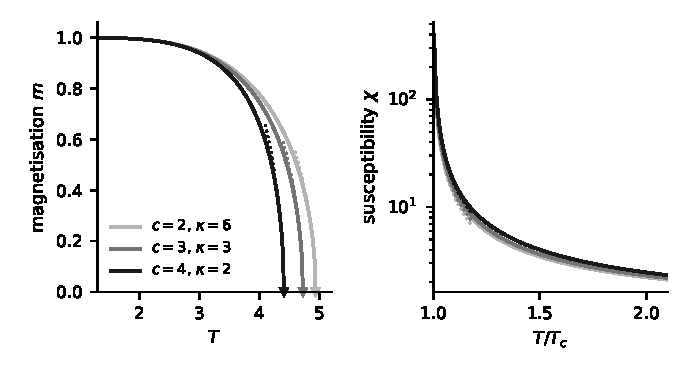
\includegraphics[width=\linewidth]{figs/fig-response.pdf}
\caption{\textbf{One formula, three interiors.} A single clique layer of
cardinality $c$ at chy-degree $\kappa$, with $\kappa(c-1)=6$ held fixed, so
every member has six neighbours either way and only what is inside a complex
differs. Left: the order parameter from Eq.~\eqref{eq:magclosure} in absolute
temperature, with the square-root asymptote Eq.~\eqref{eq:magamp} dotted and
each $T_{c}$ marked; it falls as the cardinality rises. Right: the response
from Eq.~\eqref{eq:chi} against reduced temperature, with the $\gamma=1$
asymptote Eq.~\eqref{eq:chiamp} dotted. Generated by
\code{figs/\allowbreak statmech.\allowbreak py}.}
\label{fig:response}
\end{figure}

\paragraph{What each of the two requires.} They are not equally general, and
the difference is the shape of the measure. Equation~\eqref{eq:chi} needs only
the linearisation, so it holds wherever Eq.~\eqref{eq:branch} does.
Equation~\eqref{eq:magclosure} needs the measure to be a point mass, so a
Poisson chy-degree, a fractional one, or a layer mixing cardinalities all leave
it: those carry a distribution of fields, the mean cardinality is not a summary
of one, and the route is the population. \code{Chygraph.\allowbreak
magnetisation} refuses such a structure rather than returning a number for it.

\section{The free energy from replicas}
\label{sec:replicas-chy}
\index{replica method|textbf}
\index{functional order parameter|textbf}
\index{Bethe free energy}

Sections~\ref{sec:freeenergy} and~\ref{sec:response} took the Bethe free energy
as given and differentiated it. It can instead be derived, from
Eq.~\eqref{eq:Z-intro} and nothing else, and the derivation is worth having for
what comes with it rather than for the free energy, which it returns unchanged.
It produces Eq.~\eqref{eq:bethe}'s counting numbers instead of assuming them.
It produces the two steps of Sec.~\ref{sec:twosteps}, excess bracket included,
as a stationarity condition instead of as bookkeeping put in by hand. And it
defines an order parameter \emph{before} any assumption about the number of
states, which is the object Sec.~\ref{sec:onestep} then breaks the symmetry of.

The calculation is \citet{leone2002}'s for a graph and
\citet{vazquez2003vw}'s with degree correlations, carried to a chygraph. The
formalism is \citet{mezard1987}; the diluted case in the form used here is
\citet{franz2003}.

One note on letters. In this section $n$ is the number of replicas and
$r=1,\dots,n$ indexes them, which is the only place in the book either does
that job; $\vec\sigma_{i}=(\sigma^{1}_{i},\dots,\sigma^{n}_{i})$ collects the
$n$ copies of the variable at atom $i$.

\paragraph{The object to average.} Take one atom layer and $L$ complex layers,
layer $l$ carrying cardinality $c_{l}$ and interior weight
$\chi_{l}=e^{-\beta H_{l}}$ --- the same $-\beta H$ Eq.~\eqref{eq:emitted} sums.
Then Eq.~\eqref{eq:Z-intro} reads
\begin{equation}
  Z=\sum_{\{\sigma\}}\ \prod_{i}e^{\beta B\sigma_{i}}
    \prod_{l}\prod_{a\in l}\chi_{l}\bigl(\{\sigma_{j}\}_{j\in a}\bigr),
  \label{eq:Zchy}
\end{equation}
and the free energy is $-\beta f=\overline{\ln Z}/N$, the bar an average over
which atoms each complex holds. That average is what the replica identity of
Sec.~\ref{sec:replicas} is for: $\overline{\ln Z}=\lim_{n\to0}
(\overline{Z^{n}}-1)/n$, with
\begin{equation}
  \overline{Z^{n}}=\sum_{\{\vec\sigma\}}\prod_{i}
    e^{\beta B\sum_{r}\sigma^{r}_{i}}\ \
    \overline{\prod_{l}\prod_{a\in l}\prod_{r}
      \chi_{l}\bigl(\{\sigma^{r}_{j}\}_{j\in a}\bigr)}.
  \label{eq:Zn}
\end{equation}
The chy-degrees are prescribed, so the average carries one constraint per atom
per layer, written in the integral form
$\delta\bigl(\sum_{a\in l}\alpha_{ia}-\kappa^{l}_{i}\bigr)
=\int\frac{\mathrm{d}\psi^{l}_{i}}{2\pi}
 e^{\mathrm{i}(\sum_{a\in l}\alpha_{ia}-\kappa^{l}_{i})\psi^{l}_{i}}$
with $\alpha$ the chy-adjacency matrix of Eq.~\eqref{eq:alpha}. This is the one
place a chygraph costs more than a graph: an edge is a pair by construction, so
a graph needs this constraint once, while a complex has a cardinality of its own
and needs it on both margins of $\alpha$.

\paragraph{The order parameter.} Tracing over the variables and integrating out
the $\psi$'s leaves everything expressed through one function per layer,
\begin{equation}
  \rho_{l}(\vec\sigma)=\frac{1}{N}\sum_{i}
     \delta_{\vec\sigma,\vec\sigma_{i}}\ e^{\mathrm{i}\psi^{l}_{i}},
  \label{eq:rhochy}
\end{equation}
and its conjugate $\hat\rho_{l}(\vec\sigma)$. It is a distribution over the
$2^{n}$ replica states, resolved by layer, and it is a \emph{functional} order
parameter: not a number, and not yet a field. Nothing has been assumed about it.
With
\begin{equation}
  \Xi_{l}[\rho]=\!\!\sum_{\vec\sigma_{1}\dots\vec\sigma_{c_{l}}}\
    \prod_{j=1}^{c_{l}}\rho_{l}(\vec\sigma_{j})
    \prod_{r}\chi_{l}\bigl(\sigma^{r}_{1},\dots,\sigma^{r}_{c_{l}}\bigr)
  \label{eq:Xichy}
\end{equation}
the interior sum in replica space, $\overline{Z^{n}}=\int\prod_{l,\vec\sigma}
\mathrm{d}\rho_{l}\,\mathrm{d}\hat\rho_{l}\ e^{-nNF}$ with
\begin{equation}
  \begin{aligned}
  -nF=&-\sum_{l}\ave{\kappa_{l}}\sum_{\vec\sigma}
        \rho_{l}(\vec\sigma)\hat\rho_{l}(\vec\sigma)\\
      &+\Bigl\langle\ln\sum_{\vec\sigma}e^{\beta B\sum_{r}\sigma^{r}}
        \prod_{l}\hat\rho_{l}(\vec\sigma)^{\kappa_{l}}\Bigr\rangle
       +\sum_{l}\frac{\ave{\kappa_{l}}}{c_{l}}\,\Xi_{l}[\rho],
  \end{aligned}
  \label{eq:Fchy}
\end{equation}
additive constants dropped.

\paragraph{What the three terms are.} They are one per complex, one per atom and
one subtracted per inclusion --- which is Sec.~\ref{sec:freeenergy}'s
un-collapsed free energy, term for term. The complex term carries
$\ave{\kappa_{l}}/c_{l}$, which is Eq.~\eqref{eq:bethe}'s $n_{l}$: a chygraph
has that many layer-$l$ complexes per atom. The inclusion term carries
$\ave{\kappa_{l}}$, one per inclusion. So Eq.~\eqref{eq:bethe}'s counting
numbers are not a choice made to make a tree work. They are the structure of
Eq.~\eqref{eq:Fchy}, and they were already the M\"obius numbers of
Chapter~\ref{ch:gbp}'s region graph. Three routes, one set of weights.

\paragraph{The saddle point is the two steps.} Setting the variations of
Eq.~\eqref{eq:Fchy} to zero gives
\begin{align}
  \hat\rho_{l}(\vec\sigma)&=\!\!\sum_{\vec\sigma_{2}\dots\vec\sigma_{c_{l}}}
    \prod_{j=2}^{c_{l}}\rho_{l}(\vec\sigma_{j})
    \prod_{r}\chi_{l}\bigl(\sigma^{r},\sigma^{r}_{2},\dots,
      \sigma^{r}_{c_{l}}\bigr),\label{eq:saddledown}\\
  \rho_{l}(\vec\sigma)&=\Bigl\langle\frac{\kappa_{l}}{\ave{\kappa_{l}}}\,
    \frac{e^{\beta B\sum_{r}\sigma^{r}}\hat\rho_{l}(\vec\sigma)^{\kappa_{l}-1}
          \prod_{m\ne l}\hat\rho_{m}(\vec\sigma)^{\kappa_{m}}}
         {\sum_{\vec\sigma'}e^{\beta B\sum_{r}\sigma'^{r}}
          \prod_{m}\hat\rho_{m}(\vec\sigma')^{\kappa_{m}}}\Bigr\rangle.
  \label{eq:saddleup}
\end{align}
Read them against Sec.~\ref{sec:twosteps}. Equation~\eqref{eq:saddledown} is the
down step: a complex reports what its other $c_{l}-1$ members do, summed over
its interior exactly. Equation~\eqref{eq:saddleup} is the up step, and it
carries two things that Sec.~\ref{sec:map} put in by hand. The weight
$\kappa_{l}/\ave{\kappa_{l}}$ is the size-biasing of
Sec.~\ref{sec:branching} --- a complex is reached in proportion to how many
inclusions it has. And the exponent is $\kappa_{l}-1$ in the layer arrived
through and $\kappa_{m}$ in every other, which is the excess bracket
$[\bar\Phi]_{k=m}$ of Fig.~\ref{fig:themap}. Neither was an assumption. Both
are what stationarity returns.

\paragraph{Replica symmetry, and Eq.~\eqref{eq:bethe}.} Write
$\nu_{h}(\sigma)$ for the normalised one-site law that a message $h$ stands
for: $e^{h\sigma}/2\cosh h$ for an Ising spin, a distribution over $q$ colours
in Chapter~\ref{ch:colouring}, a warning in
Chapter~\ref{ch:satisfiability}. What a message \emph{is} is the only thing
that changes from model to model, and Sec.~\ref{sec:onestep} is where it decides
what the next step costs. The replica-symmetric ansatz is then that a replica
state is a superposition of product states weighted by one message,
\begin{equation}
  \rho_{l}(\vec\sigma)=\!\int\!\mathrm{d}h\,P_{l}(h)
    \prod_{r}\nu_{h}(\sigma^{r}),
  \qquad
  \hat\rho_{l}(\vec\sigma)=\!\int\!\mathrm{d}u\,Q_{l}(u)
    \prod_{r}\nu_{u}(\sigma^{r}),
  \label{eq:rsansatz}
\end{equation}
which is where a message first enters the calculation --- and it enters as an
ansatz, not as a definition. Substituting Eq.~\eqref{eq:rsansatz} into
Eq.~\eqref{eq:saddledown} makes $Q_{l}$ the law of the field a complex emits
when its other members carry fields drawn from $P_{l}$, and the emitted field is
Eq.~\eqref{eq:emitted}. Substituting into Eq.~\eqref{eq:saddleup} makes $P_{l}$
the law of $B$ plus the fields arriving from the other complexes, which is the
convolution Eq.~\eqref{eq:ensemblemap}. Substituting into Eq.~\eqref{eq:Fchy}
returns Eq.~\eqref{eq:bethe}. So the whole of this chapter up to
Sec.~\ref{sec:response} is Eq.~\eqref{eq:Fchy} under one ansatz, and at
$c_{l}=2$ and one layer it is \citeauthor{leone2002}'s graph result.

\paragraph{The stability line, derived.} Expanding Eq.~\eqref{eq:Fchy} to second
order about the replica-symmetric saddle splits the fluctuations into sectors
that do not mix, classified by how they transform under permutations of the
replicas, and the one that goes unstable first is the \emph{replicon}. Its
eigenvalue is Eq.~\eqref{eq:branch} with $u'$ replaced by $u'^{2}$, which is the
elementwise reweighting of Eq.~\eqref{eq:reweight} and so
Sec.~\ref{sec:atline}'s de~Almeida--Thouless line. That section reaches the same
condition from the argument that a perturbation of random sign is transmitted
with $u'$ and its effect measured by squaring. The Hessian route is the one that
would establish it rather than motivate it, and the sectors are named here
without being computed.

\paragraph{What this does not do.} It does not make one-step replica symmetry
breaking cheap. Equation~\eqref{eq:Fchy} is the object a one-step ansatz acts
on, and Sec.~\ref{sec:onestep} writes that ansatz down; what neither supplies is
a solution where the message is a real field rather than a warning.
Section~\ref{sec:hsrsb} is where that is met and declined, and
Sec.~\ref{sec:notdone} lists it. The derivation moves the difficulty from
\emph{what object to write} to \emph{how to solve it}, which is progress of a
limited kind and is worth saying plainly.

\section{One step of replica symmetry breaking}
\label{sec:onestep}
\index{replica symmetry breaking!one-step, on a chygraph|textbf}
\index{survey propagation|textbf}
\index{complexity|textbf}
\index{Parisi parameter}

Everything above carries one field per inclusion, and that is an assumption
about the solution space and not a convention. A message can be a field because
there is one thing to say. Where the space shatters into exponentially many
clusters --- as it does for every hard constraint in Part~III, at a density
below the one where solutions disappear --- each cluster would send its own
field along the same inclusion, and no single field is right for all of them.

\paragraph{The substitution, one level up.} The repair is
Sec.~\ref{sec:substitution}'s move made a second time, and it is worth being
exact about the difference, because the two produce the same kind of object for
different reasons. There, a field became a \emph{measure over fields} to pass
from one realisation to an ensemble: the spread in $P^{ml}$ is variation across
the graphs in the ensemble. Here a field becomes a measure over fields at
\emph{fixed} realisation: the spread is variation across the clusters of one
graph. That object is a \emph{survey},
\begin{equation}
  S_{i\to a}(h)=\text{the law, over clusters, of the field }i\text{ sends }a,
  \label{eq:survey}
\end{equation}
and the ensemble version stacks on top of it --- a distribution over surveys,
which is what a population dynamics stores and why the populations of
Chapters~\ref{ch:colouring} and~\ref{ch:satisfiability} are populations of
distributions rather than of numbers.

What does \emph{not} change is the recursion. The up step of
Sec.~\ref{sec:upstep} still adds the incoming fields; the down step of
Sec.~\ref{sec:downstep} still enumerates the interior of a complex exactly.
Both now act on surveys rather than on fields, and each combination is
reweighted by $e^{-m\Delta F}$, with $\Delta F$ the free-energy shift the
combination costs and $m$ the Parisi parameter --- the one place in this chapter
where $m$ is not a layer index. The index structure --- layers,
the direction of arrival, the discounting of the inclusion one came in by ---
survives this exactly as it survived the first substitution, and for the same
reason: none of it was ever about what the message contained.

\paragraph{Counting the clusters.} A branch of the survey recursion appearing is
not a threshold. What decides whether solutions still exist is how many clusters
there are, and that is a free energy rather than a branch. Reweighting
Eq.~\eqref{eq:bethe} at $m=0$ turns the Bethe expression into a count of
clusters --- the \emph{complexity}
\begin{equation}
  \Sigma=\ave{\ln Z_{i}}
        +\sum_{l}\frac{\ave{\kappa_{l}}}{c_{l}}\ave{\ln Z^{(l)}_{a}}
        -\sum_{l}\ave{\kappa_{l}}\ave{\ln Z^{(l)}_{ia}},
  \label{eq:sigmagen}
\end{equation}
the same three objects the free energy is built from --- a node, a complex, an
inclusion --- evaluated on surveys instead of on fields, with
$\ave{\kappa_{l}}/c_{l}$ complexes and $\ave{\kappa_{l}}$ inclusions per node in
layer $l$. Where $\Sigma$
falls to zero the clusters have run out, and that is the threshold. Note that
the overlap term does not collapse here as it did in
Eq.~\eqref{eq:bethe}: the argument that made $h_{i\to a}+u_{a\to i}$ the same
full field for every complex is an argument about one field, and the
reweighting is what breaks it. Three terms rather than two is the whole
bookkeeping cost of the step.

\paragraph{The same step, on the replica order parameter.}
Equation~\eqref{eq:survey} is a definition, and
Sec.~\ref{sec:replicas-chy} says what it is an ansatz \emph{for}. Replica
symmetry was Eq.~\eqref{eq:rsansatz}, every replica carrying the same field.
Break the $n$ replicas into $n/m$ blocks of $m$, let the field be common within
a block and drawn from a distribution across blocks, and
Eq.~\eqref{eq:rhochy} becomes
\begin{equation}
  \rho_{l}(\vec\sigma)=\int\!\mathcal{D}Q\ \mathcal{P}_{l}[Q]
    \prod_{\text{blocks}}\Bigl[\int\!\mathrm{d}h\,Q(h)
      \prod_{r\in\text{block}}\nu_{h}(\sigma^{r})\Bigr],
  \label{eq:rsbansatz}
\end{equation}
with $Q$ the survey of Eq.~\eqref{eq:survey} and $\mathcal{P}_{l}$ the law over
surveys that the ensemble carries. Two things then follow instead of being
imposed. The reweighting $e^{-m\Delta F}$ is what the sum over blocks produces,
so $m$ is a block size rather than a parameter added to taste. And substituting
Eq.~\eqref{eq:rsbansatz} into Eq.~\eqref{eq:Fchy} returns
Eq.~\eqref{eq:sigmagen}, which also says why the overlap term does not collapse
here as it did in Eq.~\eqref{eq:bethe}: that collapse used one field per
inclusion, and Eq.~\eqref{eq:rsbansatz} carries a distribution of them.

\paragraph{Two transitions, not one.} The survey recursion therefore carries two
pieces of information and they should not be confused. The trivial survey ---
every cluster sending the same field, which is the replica-symmetric solution
--- is a fixed point at any density. Where a second branch appears, the state
space has \emph{shattered}: there are now many clusters, and that density is the
dynamical or clustering transition. Where $\Sigma$ then falls to zero the
clusters have run out and solutions cease to exist. Solutions survive past the
first and not past the second, and the gap between them is the r\'egime survey
propagation was invented for.

The first of the two is sometimes reachable without a survey at all. Where the
shattering coincides with the appearance of a rigid structure, that structure
can be found by an ordinary percolation calculation of the kind Part~II
supplies: Chapter~\ref{ch:cover}'s core is exactly this, located by algebra
rather than by a population, and Chapter~\ref{ch:colouring} finds the same class
of point as the onset of its survey branch. The structural route is cheaper and
exact, and it is model-specific --- it says where clusters appear and nothing
about how many, which is what $\Sigma$ is for.

\paragraph{$m=0$, and what it buys.} Setting $m=0$ weights every cluster
equally, which is the right choice for counting clusters of \emph{zero-energy}
solutions and the wrong one for anything finer. There the reweighting is trivial
except at one place --- a combination that contradicts itself gets weight zero
and is discarded --- and the recursion reduces to \emph{survey propagation}.
This is the form Part~III uses, in Secs.~\ref{sec:colouring-sp}
and~\ref{sec:sat-sp}, and Eq.~\eqref{eq:sigmagen} is the equation both of those
sections instantiate. What $m=0$ does not reach is the condensation and rigidity
transitions, which need $m\ne0$ and are outside this book.

\paragraph{What the step costs.} Three things, and the last is the one a
chygraph makes visible.

\emph{The scalar closure goes.} Under replica symmetry a hard-field message is
present or absent and its mean is all of it, so a single number closes the
recursion over an ensemble. A survey is a continuous variable and its
\emph{spread} enters the next update; solving for the mean alone is not an
approximation but a different and wrong calculation.
Section~\ref{sec:sat-sp} measures the error at $28$ per cent.

\emph{The alphabet decides whether it is affordable at all.} Where the
underlying message is a warning --- present or absent, or one of a few discrete
states, which is what a hard constraint at zero temperature produces --- a
survey is a distribution over a finite alphabet and can be carried as a handful
of numbers. Where the message is a real field, a survey is a distribution over
distributions, and the population becomes a population of populations. That is
the line this book does not cross: Chapters~\ref{ch:colouring}
and~\ref{ch:satisfiability} are the two problems whose messages are warnings,
and Sec.~\ref{sec:hsrsb} is where the heavier object is met and declined.

\emph{The interior sum grows, by an amount the model decides.} The cost of
Eq.~\eqref{eq:emitted} was $2^{c}$ and depended on nothing but cardinality. The
cost of the same sum on surveys depends on how much one complex can transmit at
once. Where a complex can force at most one thing --- the hypergraph rule of
Sec.~\ref{sec:colouring-sp-chy}, a $k$-SAT clause --- the message is the same
kind of object it was at $c=2$ and cardinality enters through a single scalar.
Where a complex can force up to $c-1$ things at once, as proper colouring can,
the message becomes a \emph{set} and the interior must be summed over subsets;
Sec.~\ref{sec:colouring-cq} is that calculation and the extra work is real.
The distinction has no counterpart on a graph, where a complex with two members
has no room to force two things at once --- one more instance of the pattern
Sec.~\ref{sec:twoconstraints-col} collects, that cardinality two is degenerate
and a good deal of what reads as general theory is an artefact of working
there.

\section{What the scheme assumes}
\label{sec:assumes}
\index{replica symmetry breaking}

Three assumptions, of quite different weights.

\emph{Treelikeness, at the level of atoms.} Equation~\eqref{eq:up} treats an
atom's complexes as independent, which is exact when they meet in at most one
atom. This is Sec.~\ref{sec:treelike}'s condition, and it is the one
Chapter~\ref{ch:overlap} takes up: what happens when the cliques of a real
network share edges rather than vertices.

\emph{Replica symmetry.} One field per inclusion presumes a single pure state.
Equation~\eqref{eq:rsansatz} is that presumption written down, and
Sec.~\ref{sec:replicas-chy} is where it can be seen as an ansatz on something
more general rather than as the definition of a message.
Section~\ref{sec:onestep} is what replaces it where the state space shatters,
and it is a repair rather than a limit --- but a partial one, since it is
carried out at $m=0$ throughout this book.
Chapter~\ref{ch:hittingset} is where the assumption first becomes unavoidable,
and it is also where the diagnostic of Sec.~\ref{sec:fixedpoint} is needed.

\emph{An enumerable interior.} Equation~\eqref{eq:emitted} costs $2^{c}$. For
the motifs one finds in data that is nothing, and for a complex of thirty
members it is fatal. The formalism does not degrade gracefully here: it either
enumerates the interior or it does not apply. Cardinality is the one parameter
of a chygraph that has a hard ceiling, and Sec.~\ref{sec:onestep} lowers it
again wherever the interior has to be summed over surveys rather than fields.

\paragraph{A note on the numbers quoted.} Agreements reported in this book to
eight, ten or twelve digits are between two evaluations of the \emph{same}
analytic object --- a closed form against an enumeration, a symbolic derivative
against a numerical one. They establish that the implementation is faithful, not
that the physics is right. Where something is tested against something outside
the formalism it is said so: the Monte Carlo of Chapter~\ref{ch:ising}, the
leaf-removal simulations of Chapters~\ref{ch:cover} and~\ref{ch:overlap}, the
configuration-model simulations of Chapter~\ref{ch:giant}, and published values
where they exist. The distinction matters most in exactly this chapter, which
has nothing in it to compare against experiment and everything in it to get
wrong.

\section{Checks}
\label{sec:statmech-checks}

\checkhead{Known results}
Equation~\eqref{eq:bethe} is evaluated on populations produced by iterating
Eq.~\eqref{eq:ensemblemap} itself, then compared with the closed form of
Eq.~\eqref{eq:para} and with the textbook Bethe expression
$\ln2+(\ave{k}/2)\ln\cosh\beta J$ for a graph. The three agree to ten digits, and the
outermost of them is a simulation of the distributions rather than an evaluation
of a formula.

\checkhead{New results}
Nothing else in this chapter has appeared elsewhere, so the checks are against
independent evaluations of the same object.
Section~\ref{sec:response}'s two observables are checked as limits rather than
at a point: $m/(1-T/T_{c})^{1/2}$ against $A_{m}$ and $\chi\,(T/T_{c}-1)$
against $A_{\chi}$, over three decades of reduced temperature and on five
structures, agreeing to a part in a thousand at the closest, so the exponents
$\beta=1/2$ and $\gamma=1$ are measured rather than asserted. That $1/\chi$
vanishes exactly where $\det(I-B)$ does is checked on four layer lists rather
than argued from Eq.~\eqref{eq:chicav}. Equation~\eqref{eq:mfromZ} asserts one
thing the derivation does not enforce, that the response is the field
derivative of the order parameter, and it is checked directly: the closed form
Eq.~\eqref{eq:chi} against a finite difference of Eq.~\eqref{eq:magclosure} in
the field, on four structures at three temperatures each, agreeing to five
digits --- the accuracy of the difference and not of either expression.
Equation~\eqref{eq:chi} is checked to be general in the cardinality
distribution by the two routes Eq.~\eqref{eq:sbaru} is: a mixed layer against
the same layer split into one layer per cardinality, agreeing to machine
precision at three temperatures, and against the mean-cardinality substitution,
which must not agree and does not, by $14.6$ per cent. That $u'$ is
Chapter~\ref{ch:potts}'s $\tau_{c}$ is checked directly: the symbolic
$q$-derivative of Sec.~\ref{sec:transmission}, evaluated at $q=2$ and rewritten
in $t=\tanh\beta J$, agrees with the independent enumeration behind
Eq.~\eqref{eq:emitted} for $c=2,3,4$ at every coupling tried, to machine
precision. Two chapters written from different starting points return one
number. Equation~\eqref{eq:sbaru} is checked by the two routes of
Sec.~\ref{sec:branching}: a mixed-cardinality layer against the same layer split into one
layer per cardinality, which must agree and do, to nine digits; and against the
mean-cardinality substitution, which must not agree and does not, by $10.1$ per cent.
Equation~\eqref{eq:LT} is checked against the numerical determinant of
Eq.~\eqref{eq:branch} at the critical coupling for Poisson and for regular
layers, so that the cross term is exercised in both the case where it vanishes
and the case where it does not. Equation~\eqref{eq:exchange} is checked by
taking the residual to zero along a sequence rather than at a point, with the
sequence stopped where rounding would begin to dominate; that qualification is
the difference between demonstrating an order and quoting a number that happens
to be small.

\checkhead{Partial results}
Equation~\eqref{eq:magclosure} holds only where the message measure is a point
mass, which needs a whole-number chy-degree and one cardinality per layer.
Everything else --- a Poisson layer, a fractional chy-degree, a layer mixing
cardinalities --- carries a distribution of fields and needs the population,
which is a sample and not a closed form; the routine refuses such a structure
rather than returning a number for it. Equation~\eqref{eq:chi} has no such
restriction, so the two are not equally general and the section says which is
which. Nothing in Sec.~\ref{sec:response} is tested against a simulation
here: Chapter~\ref{ch:ising} does that, on the two structures where the
closure applies and against a Monte Carlo that has never heard of a cavity
equation.
The agreements quoted above are between two evaluations of the same analytic
object, in the sense Sec.~\ref{sec:assumes} sets out. Nothing in this chapter is
tested against experiment or against an object built to violate its assumptions:
Sec.~\ref{sec:assumes}'s three --- treelikeness at the level of atoms, replica
symmetry, and an enumerable interior --- are assumed throughout and checked
nowhere here. The one-step scheme of Sec.~\ref{sec:onestep} is written at $m=0$
only.
Section~\ref{sec:replicas-chy} is a derivation and not a computation. It
returns Eq.~\eqref{eq:bethe}, which is checked above, and adds no number of its
own. The reductions it claims --- Eq.~\eqref{eq:saddledown} to
Eq.~\eqref{eq:emitted}, Eq.~\eqref{eq:saddleup} to
Eq.~\eqref{eq:ensemblemap}, and Eq.~\eqref{eq:Fchy} to Eq.~\eqref{eq:bethe}
under Eq.~\eqref{eq:rsansatz} --- are stated as algebra and are not
machine-checked, which is a weaker footing than the rest of the chapter stands
on. Equation~\eqref{eq:rsbansatz} is written and not solved.
